\documentclass[12pt]{article}
\textwidth 15.5cm \oddsidemargin 0cm \topmargin -1cm \textheight
24cm \footskip 1.5cm \usepackage{epsfig}
\usepackage{amsmath, amsfonts, graphicx, psfrag, pstcol, float, listings}
\def\n{\noindent}
\def\u{\underline}
\def\hs{\hspace}
\newcommand{\thrfor}{.^{\displaystyle .} .}
\newcommand{\bvec}[1]{{\bf #1}}
\newcommand{\code}[1]{\texttt{#1}}

\begin{document}

\noindent
\rule{15.7cm}{0.5mm}


\begin{center}
{\bf ENGINEERING TRIPOS PART II A}
\end{center}
\vspace{0.5cm} {\bf EIETL \hfill 3F3 FULL TECHNICAL REPORT}
\vspace{0.5cm}
\begin{center}
{\bf RANDOM VARIABLES and RANDOM NUMBER GENERATION\\
Name: Harry Sarson \\\hfill\\
College: Pembroke \\\hfill
\\
Date: ????????????????????????????	
}
\end{center}
\rule{15.7cm}{0.5mm}

\pagebreak

\section{Uniform and normal random variables.}

When creating a histogram plot of random samples taken from a distribution, the probability of the histogram is given by:

\begin{equation}
    p(n_1, n_2, \ldots, n_J) = \frac {N!} {n_1! n_2! \ldots n_J!} p_1^{n_1} p_2^{n_2} \ldots p_j^{n_J}
\end{equation}

Where $N = \sum n_j$. For the $j^{th}$ sample from the distribution there is a probability, $p_j$, that the sample will fall into the $j^{th}$ bin.
Therefore, when $N$ samples are taken from the distribution the probability that there are $n_j$ in the $j^{th}$ bin is given by the binomial distribution

\section{Functions of random variables}

\subsection{$X \sim {\cal N}(x|0,1)$}

Take ${Y_1} = f(X) = aX + b$, and so $f^{-1}(y) = (y - b) / a$ .
\begin{align}
p_{Y_1}(y) &= \left. \frac {p_X(x)} {\frac {dy} {dx}} \right|_{x = f^ {-1} (y)} \nonumber \\
p_{Y_1}(y) &= \frac 1 a  {p_X \left (\frac {y - b} a \right)}
\end{align}
Therefore $Y_1 \sim {\cal N}(y|b, a^2)$ and so a linear function of a Gaussian random variable with zero mean and unit variance creates a general normal density with non-zero mean and non-unity variance.

Now take $Y_2 = f(x)=x^2$. Therefore, $\frac{dy}{dx} = 2x$  and $f^{-1}(y) = \pm \sqrt{y}$. Note $f^{-1}(y)$ is multivalued with ${f_1}^{-1}(y) = \sqrt{y}$ and ${f_2}^{-1}(y) = -\sqrt{y}$.

\begin{alignat*}{2}
  p_{Y_2}(y)  
  &= \left. \frac {p_X(x)} {\left| \frac {dy} {dx} \right|} \right|_{x = {f_1} ^ {-1} (y)}
  && + \left. \frac {p_X (x)} {\left| \frac {dy} {dx} \right|} \right|_{x = {f_2} ^ {-1} (y)} \\
  &= \frac {p_X ( \sqrt y )} {\left| 2 \sqrt y \right|}  && + \frac {p_X (- \sqrt y)} {\left| - 2 \sqrt y \right|} \\
  p_{Y_2}(y) &\stackrel {(a)} {=} \frac {p_X (\sqrt y)} {\sqrt y} \\    
\end{alignat*}
\begin{equation}
  p_{Y_2}(y) = 
  \begin{cases} 
    \frac 1 {\sqrt{2 \pi y}} e ^ { - y /2} &\mbox{if } y \ge 0 \\
    \, 0 &\mbox{otherwise}
  \end{cases}
\end{equation}
Where $(a)$ follows because $p_X$ is an even function when $X$ has a Gaussian distribution.

\subsection{$X \sim {\cal U}(x|0, 2\pi)$}

Take $Y_3 = f(X) = \sin(X)$. This gives, $\frac{dy}{dx} = \cos(x) = \sqrt{1 - y^2}$  and $f^{-1}(y) = \pm \sqrt{y}$. Note $f^{-1}(y)$ is multivalued and has an infinite number of inverses. However, $p_X(x) = 0$ for $x \not\in [0, 2\pi]$ and so only three of the inverses produce non-zero terms: 

$$
{f_1}^{-1}(y) = \sin^{-1}{y}\mbox{, }{f_2}^{-1}(y) = \pi - \sin^{-1}{y}\mbox{, }{f_3}^{-1}(y) = 2\pi + \sin^{-1}{y}
$$

Notice that the range of $Y$ is $[-1, 1]$ Using the Jacobian method and summing over the solutions for $f_1$, $f_2$ and $f_3$ gives:

\begin{align}
  p_{Y_3}(y) &= \frac {p_X ( \sin^{-1} y )} {\sqrt{1 - y^2}}
  + \frac {p_X ( \pi - \sin^{-1} y )} {\sqrt{1 - y^2}}
  + \frac {p_X ( 2\pi + \sin^{-1} y )} {\sqrt{1 - y^2}} \\
  p_{Y_3}(y) &= \frac {p_X ( y ) + 1/2\pi + p_X ( -y )} {\sqrt{1 - y^2}} \\
  p_{Y_3}(y) &=
  \begin{cases} 
    \frac 1 {\pi\sqrt{1 - y^2}} &\mbox{if } -1 < y < 1 \\
    \, 0 &\mbox{otherwise}
  \end{cases}
\end{align}

Now consider the PDF of $Y_4 = \min{(Y_3, 0.7)}$.

\begin{equation}
  p_{Y_4}(Y_4 \ge y) =
  \begin{cases} 
    P_{Y_3}(Y_3 \ge y) &\mbox{if } y < 0.7 \\
    \, 1 &\mbox{otherwise}
  \end{cases}
\end{equation}

Therefore the PDF of $Y_4$ is identical to that of $Y_3$ for $y < 0.7$, has a delta function at $y = 0.7$ and is zero for $Y > 0.7$. There is a non-zero probability of samples being exactly $0.7$ which is given by:

$$
  p_{Y_4}(0.7) = 
  \int _ {0.7} ^ 1 p_{Y_3}(y) \, dy = 
  \int _ {sin^{-1}(0.7)} ^ {\pi - sin^{-1}(0.7)} p_X(x) dx =
  \frac 1 2 - \frac {sin^{-1}(0.7)} \pi \approx
  0.2532
$$

\section{Generating an exponential random variable with the inverse CDF method.}

An exponential distribution is defined by the PDF:

\begin{equation}
  p_Y(y)  = \lambda  ^ {- \lambda y}, y \ge 0	
\end{equation}

The mean and variance of the distribution are given by: $\mu = 1 / \lambda$ and $\sigma ^ 2 = 1 / \lambda ^ 2$ and the CDF $F_Y(y)$ and the inverse CDF ${F_Y}^{-1}(x)$ are given by:

\begin{align}
  F_Y (y) &= \int _ {- \infty} ^ y p_Y (y) \, dy =  \int _ 0 ^ y \lambda e ^ {- \lambda y} \, dy = 1 - e ^ {- \lambda y} \\
  {F_Y} ^ {-1} (x) &= \frac 1  \lambda \log {\left( \frac 1 {1 - x} \right)} \\
  y^{(i)} &= {F_Y} ^ {-1} (x ^ {(i)}) = \frac 1  \lambda  \log \left(\frac 1 {1 - x ^ {(i)}}  \right)
\end{align}

One way of verifying the samples are correctly distributed is to calculate estimates for the mean and variance of the samples using Monte Carlo:
\begin{align}
	\hat{\mu} &= \frac 1 N \sum ^ N _ {i=0} y^{(i)} \\
    \hat{\sigma}^2 &= \frac 1 N \sum ^ N _ {i=0} (y^{(i)})^2 - \hat \mu^2
\end{align}

This estimate is unbiased as:
\begin{equation}
	\mathbb{E}   [\hat{\mu}] = \frac 1 N \sum ^ N _ {i=0} \mathbb{E} [y^{(i)}] = \mathbb{E} [Y] = \mu
\end{equation}

The variance of the estimator is given by:
\begin{equation}
	\mathbb{E} [(\hat{\mu} - \mu)^2] =
    \frac 1 {N^2} \sum ^ N _ {i=0} \sum ^ N _ {j = 0} \mathbb{E} [y^{(i)}y^{(j)}] - \mu^2 =
   \frac {N\sigma^2 + N^2\mu^2} {N^2} - \mu^2 = 
   \frac {\sigma^2} N
\end{equation}
Because 
\begin{equation*}
  \mathbb{E} [y^{(i)}y^{(j)}]  = 
  \begin{cases} 
      \mathbb{E} [Y^2] = \sigma^2  +\mu^2 & \mbox{if } i = j \\
      \mathbb E [Y]^2 = \mu^2 & \mbox{if } i \ne j  	
  \end{cases}
\end{equation*}

Figure \ref{fig:mote-mean} shows a log-log plot of the mean squared error of the Monte Carlo estimator as a function of the number of samples.
The graph is created by averaging 20 estimations from separate sets of samples which smooths the plot.
The dashed line on the graph shows the theoretical variance of the estimator.

\begin{figure}[htb]
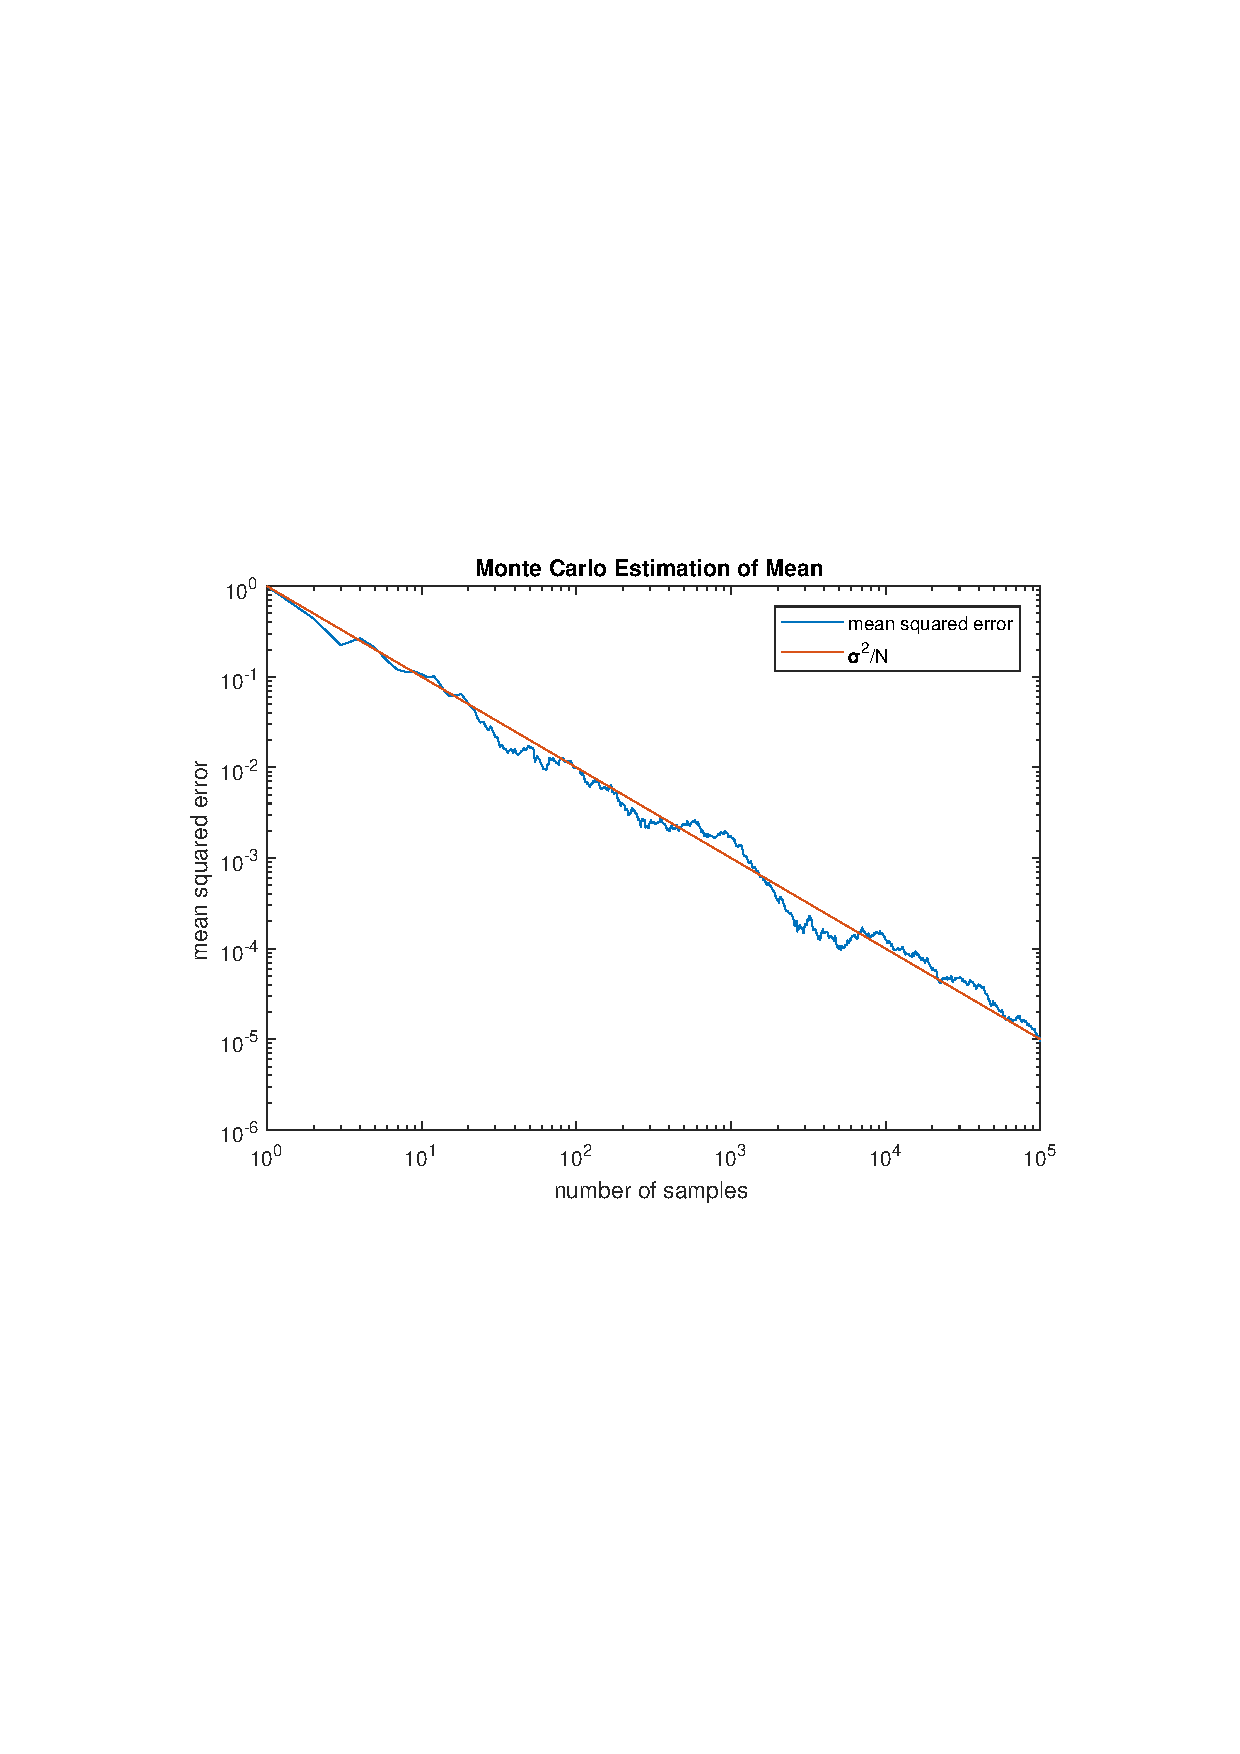
\includegraphics[width=\textwidth]{figures/mote-carlo-mean-estimator.pdf}
  \caption{???????????????}
  \label{fig:mote-mean}
\end{figure}


\end{document}



\end{document}


